\documentclass{beamer}
\usetheme{Boadilla}   
\usefonttheme[onlymath] {serif}
\definecolor {utorange} {RGB} {203,96,21}
\usecolortheme[named=utorange]{structure}
\newcommand{\vect}[1]{\boldsymbol{#1}}

      
\title{The Traffic Assignment Problem}
\subtitle{Frank-Wolfe Algortihm}
\date{October 18, 2018}
\author{Natalia Zuniga-Garcia}
\institute[UT-Austin]
{
	The University of Texas at Austin \\ 
	\medskip
	\textit{SDS 385: Statistical Models for Big Data}\\
	\medskip
	Instructor: James Scott
}

%----------------------------------------------------------------------------------------
%   TITLE PAGE
%----------------------------------------------------------------------------------------

\begin{document}
	\maketitle
	\begin{frame}
	\frametitle{Overview}
	\tableofcontents
   \end{frame}

%----------------------------------------------------------------------------------------
%   PRESENTATION SLIDES
%----------------------------------------------------------------------------------------	
	\section{The Traffic Assignment Problem}
		\begin{frame}{The Traffic Assignment Problem}
		\begin{itemize}
			\item Traffic Assignment (TA) is a process of allocating the given origin-destination (OD) trip to the transportation network under certain rules.
			\item User Equilibrium (UE) Principle: All of the used paths have equal and minimum travel times; all of the unused paths have equal or higher travel times.
			
		\end{itemize}
		 \begin{figure}
		 	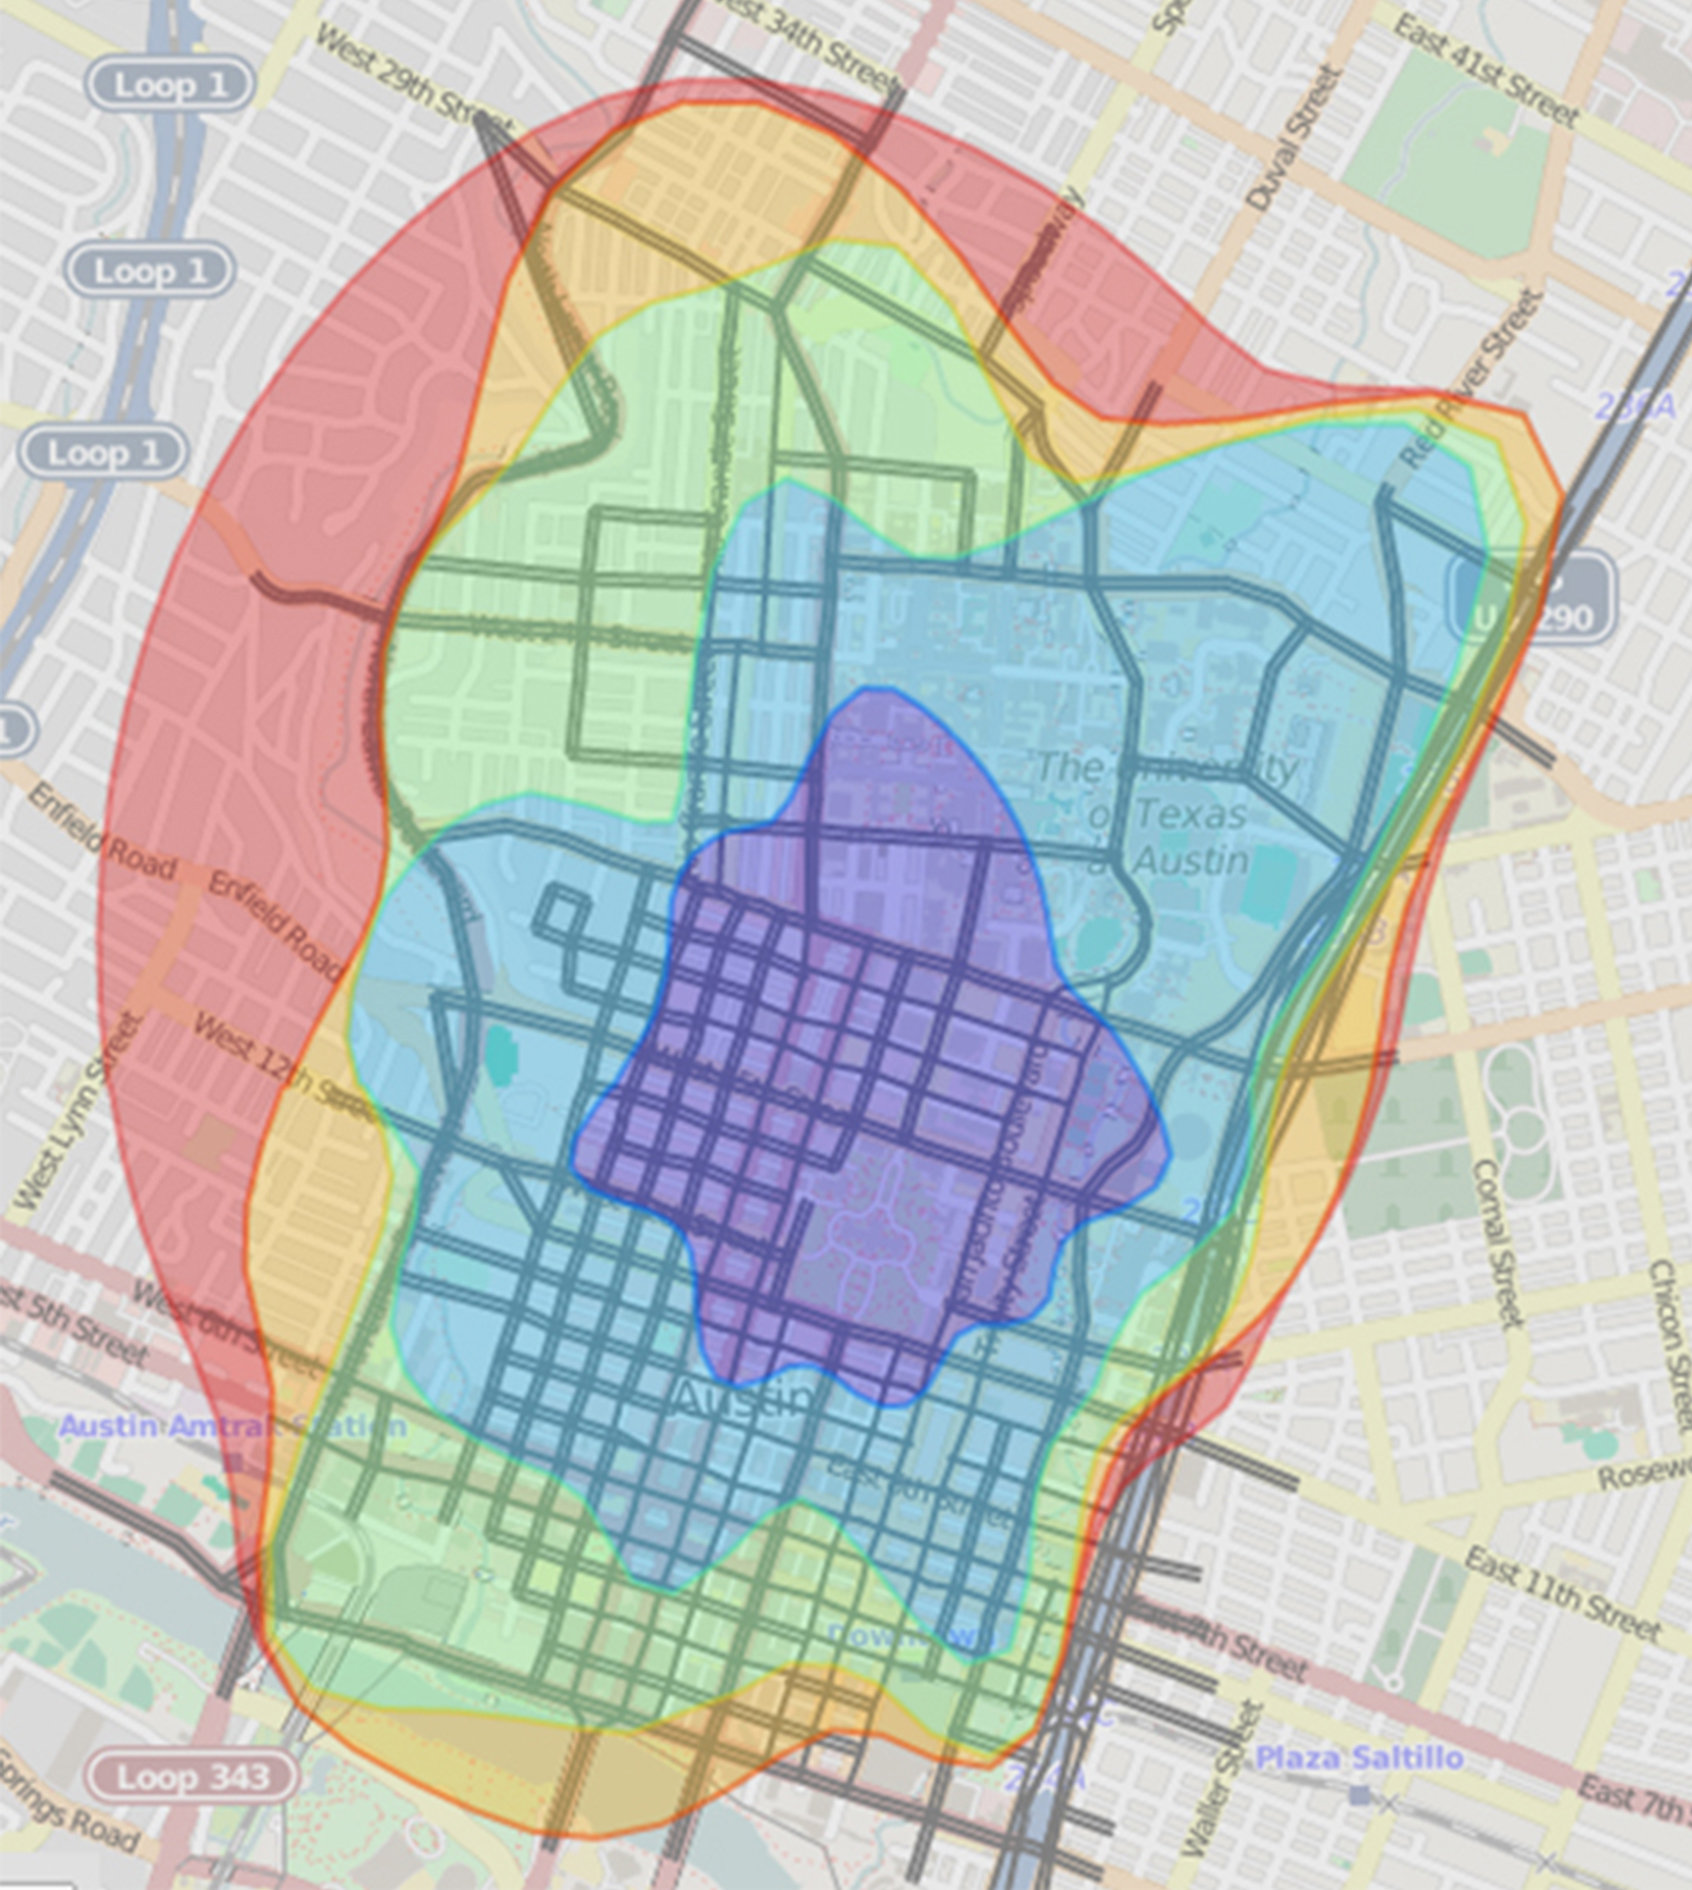
\includegraphics[width=5cm, height=4cm]{Fig/AustinTravelTime.jpg}
		 	\caption{Travel time during the morning peak in downtown Austin (UT-NMC)}
		 \end{figure}
		\end{frame}
	
%----------------------------------------------------------------------------------------		
	\section{User Equilibrium}
		\begin{frame}{User Equilibrium}
		A transportation network $G = (N, A)$ is given, where $N$ and $A$ are the sets of nodes and links, and each link  is associated
		with a positive travel time $t(x)$ as a function of link flow $x$.  For origin-destination (O-D) pair ($rs$), there is a given positive path ($\pi$) flow $h^\pi$ and its corresponding path travel time is $C^\pi$. Then, the objective function of the UE principle is \footnote{Known as the Beckmann function.}:
		$$ \min_{\vect{x},\vect{h}} \sum_{(i,j) \in A}^{} \int_{0}^{x_{ij}} \vect{t}_{ij}(x)dx$$ 
		s.t. \\
		$ \vect{h}^\pi \geq 0$  \hfill $\forall \pi \in \Pi$ \hfill Non negative path flow \\
		$ \vect{C}^\pi \geq \kappa_{rs}$  \hfill $\forall (\vect{r},\vect{s}) \in \vect{Z}^2$  \hfill $\kappa_{rs}$ is the shortest path  \\
		$ \vect{h}^\pi (\vect{C}^\pi -\kappa_{rs} ) \geq 0$  \hfill $\forall \pi \in \Pi$ \hfill If the path is use, its travel time is $\kappa_{rs}$  \\

		\end{frame} 

%----------------------------------------------------------------------------------------	
\section{Frank-Wolfe Algorithm}
\begin{frame}{Frank-Wolfe Algorithm}
	\begin{itemize}

\item Frank and Wolfe (1956) designed this conditional gradient algorithm to solve the convex quadratic problem, and LeBlanc et al. (1975) first adopted it for solution of the TA 
problem.
\item Advantages: Memory efficiency (only link variables need to be stored).
\item Disadvantage: Slow convergence near the optimal point, take long time to reach high precision.
	\end{itemize}
\begin{figure}
	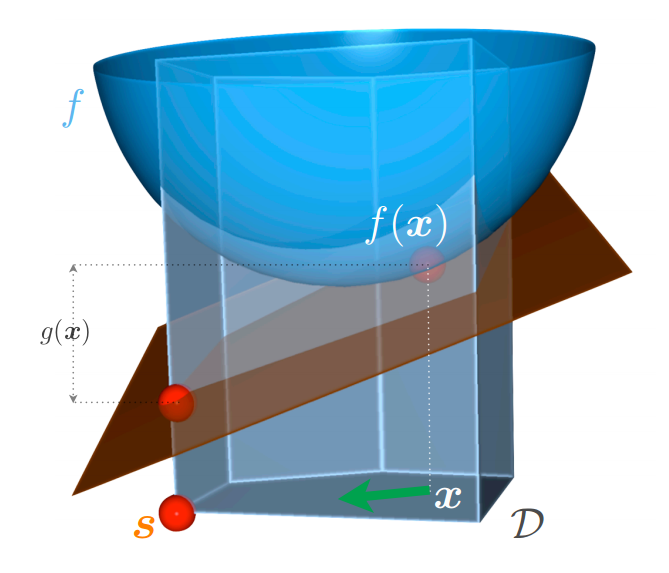
\includegraphics[width=5cm, height=4cm]{Fig/FrankWolfe.png}
	\caption{Frank-Wolfe Algorithm (Jaggi, 2013)}
\end{figure}
\end{frame}

\subsection{Application to the Traffic Assignment Problem}
\begin{frame}{Frank-Wolfe Algorithm: Traffic Assignment Problem}
	\begin{itemize}
		\item  Define $\vect{X}'=\{\vect{x}':\vect{x}=\lambda \vect{x}^{*} + (1-\lambda)\vect{x}, \lambda \in [0,1] \}$
		\item Find $\vect{x}' \in \vect{X}' $ such that $\vect{t}(x')\cdot (\vect{x}'-\vect{x}'')\leq 0$  $\forall \vect{x}'' \in \vect{X}'$
		%\item We pick a $\lambda$ to solve this, it is the same as choosing $\lambda$ to minimize the Beckmann function.
		\item We assume that the solution is not in any endpoint ($\lambda=1$ or $\lambda=1$).
		\item   Then, $\sum_{ij}^{} t_{ij}(x'_{ij})(x_{ij}^{*}-x_{ij})=0$
		\item Where, $x' = x_{ij} + \lambda(x_{ij}^{*}-x_{ij})$ or $x'=\lambda x_{ij}^{*}+(1-\lambda )x_{ij}$ 
	\begin{figure}
		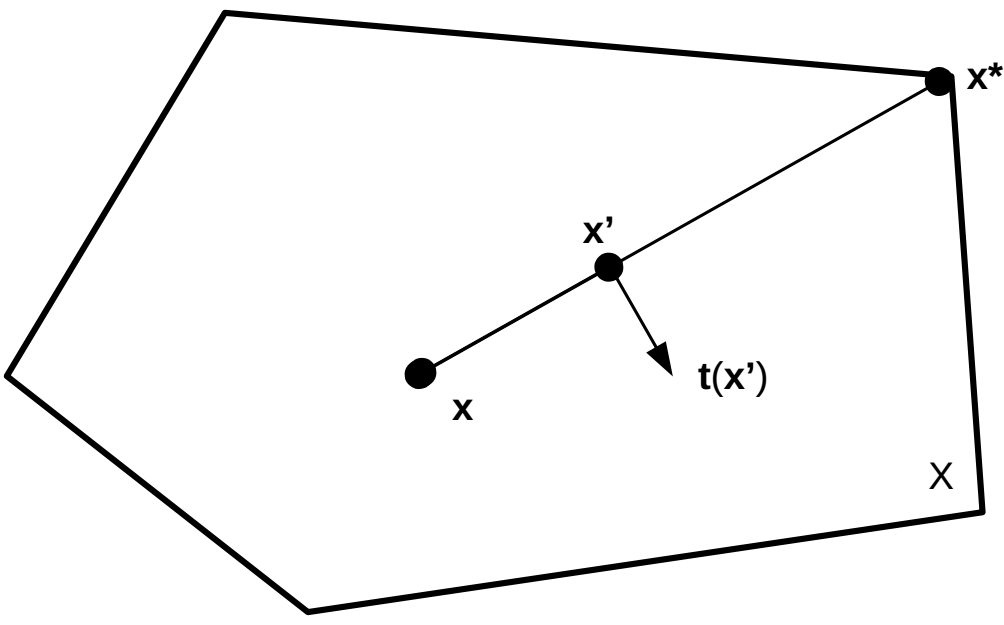
\includegraphics[width=4cm, height=4cm]{Fig/FrankWolfeSol.png}
		\caption{A solution to the Beckmann function in the FW method (Boyles, 2016)}
	\end{figure}
	\end{itemize}
\end{frame}

\subsection{Case Study: Computational Efficiency in Large Networks}
\begin{frame}{Frank-Wolfe Algorithm: Large Networks Case Study}
\begin{itemize}
	\item  Lee et al. (2002) evaluated the FW computational performance in mid- to large-scale randomly generated grid networks.
	\item Path-based algorithm:, gradient projection (GP) and disaggregate simplicial decomposition (DSD), 
	\item Link-based algorithms: Frank–Wolfe (FW), PARTAN (PT), and restricted simplicial decomposition (RSD)
	\begin{figure}
		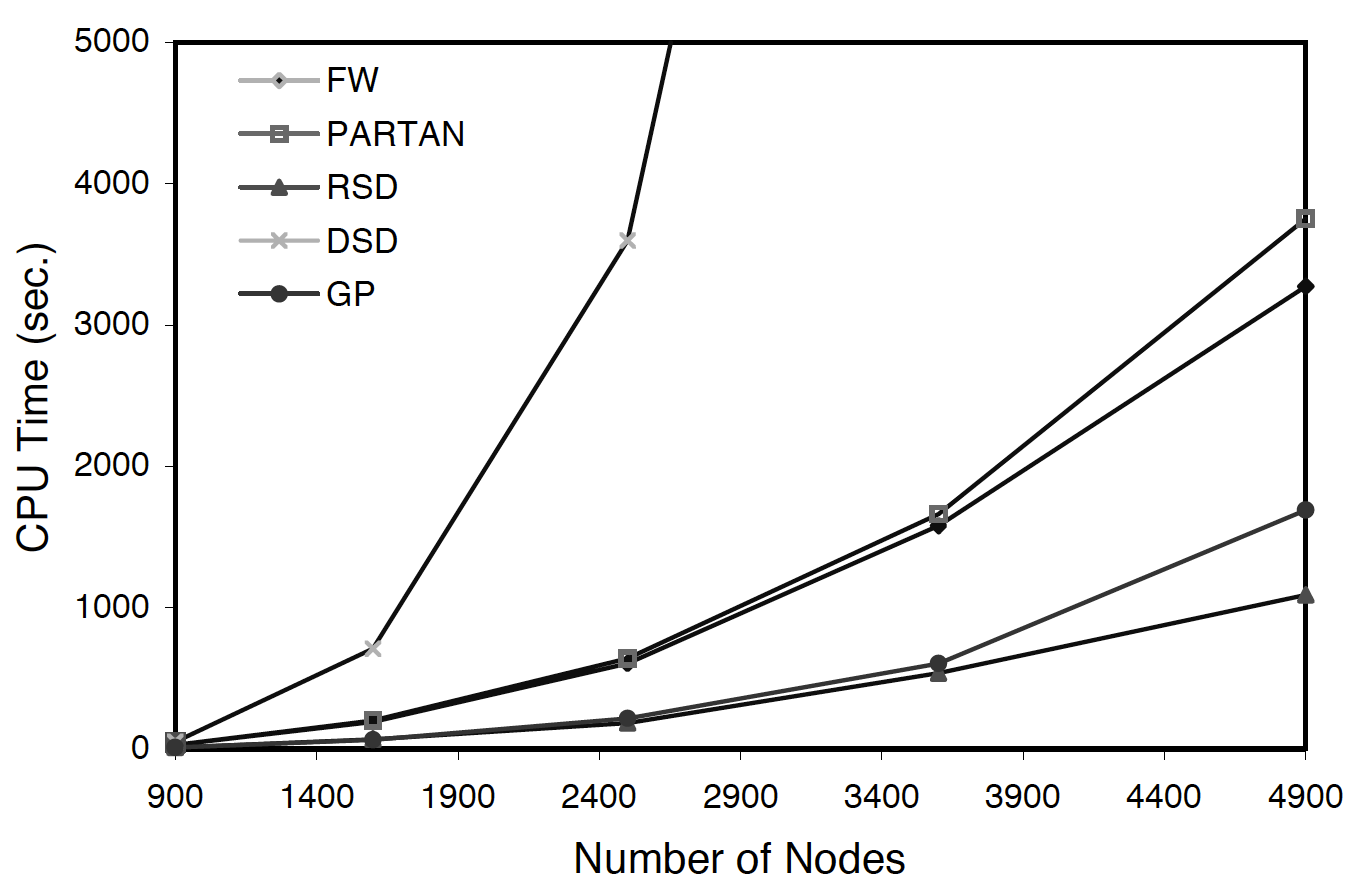
\includegraphics[width=8cm, height=4.2cm]{Fig/ComputationalTime.png}
		\caption{CPU time versus network size (Lee at al., 2002)}
	\end{figure}
\end{itemize}

\end{frame}	
%----------------------------------------------------------------------------------------	
	\begin{frame}{}
		\Huge{\centerline{Thank You!}}
		\vspace{5mm}
		\small\centerline{Questions or Comments?}
	\end{frame}

%----------------------------------------------------------------------------------------
	\begin{frame}
	\frametitle{References}
	\footnotesize{
		\begin{thebibliography}{80} 
			\bibitem[Boyles, 2016]{p1} Boyles, S. (2016).
			\newblock Transportation Network Analysis 
			\newblock \emph{Course Notes}, The University of Texas at Austin.
			\bibitem[Wolfe]{p1}Frank, M., and P. Wolfe. (1956).
			\newblock An Algorithm for Quadratic Programming. 
			\newblock \emph{Naval Research Logistics Quarterly}, Vol. 3, 1956, pp. 95–110.
			\bibitem[Wolfe]{p1}Jaggi, M. (2013, June).
			\newblock Revisiting Frank-Wolfe: Projection-Free Sparse Convex Optimization.  
			\newblock \emph{In ICML (1)}, (pp. 427-435).
			\bibitem[Lee, 2002]{p1} LeBlanc, L. J., E. K. Morlok, and W. P. Pierskalla. (1975).
			\newblock An Efficient Approach to Solving the Road Network Equilibrium Traffic Assignment Problem.
			\newblock \emph{Transportation Research Record}, Vol. 9, 1975, pp. 309–318.
			\bibitem[Lee, 2002]{p1} Lee, D., H. Nie, Y. Chen, and Leow, Y.C. (2002).
			\newblock Link and Path-Based Traffic Assignment Algorithms: Computational and Statistical Study
			\newblock \emph{Transportation Research Record} 1783, 80-88.
		\end{thebibliography}
	}
	\end{frame}
%----------------------------------------------------------------------------------------
\end{document}

